\chapter{Problem Analysis}
This chapter deals with the overall analysis of the problem itself. In the very beginning, we present the definition of the problem. Every aspect of the problem is further discussed in detail along with a comparison of possible solutions. Moreover, the next section of the chapter describes data we work with and their alternatives. The final part of this chapter presents some of the important related works.

\section{Problem definition}
First of all, we need to define the problem we are solving. The problem is defined as follows. At the input we are given an X-ray image of the patient and our goal is then to generate a corresponding textual report that will describe in detail every important aspect of the given radiograph, in particular it will describe as much as possible all the diseases actually present in the radiograph. Figure \hyperref[fig01:ProblemExample]{1.1} depicts an example of our problem with a chest X-ray image along with its ground truth and predicted report. 

\begin{figure}[h]\centering
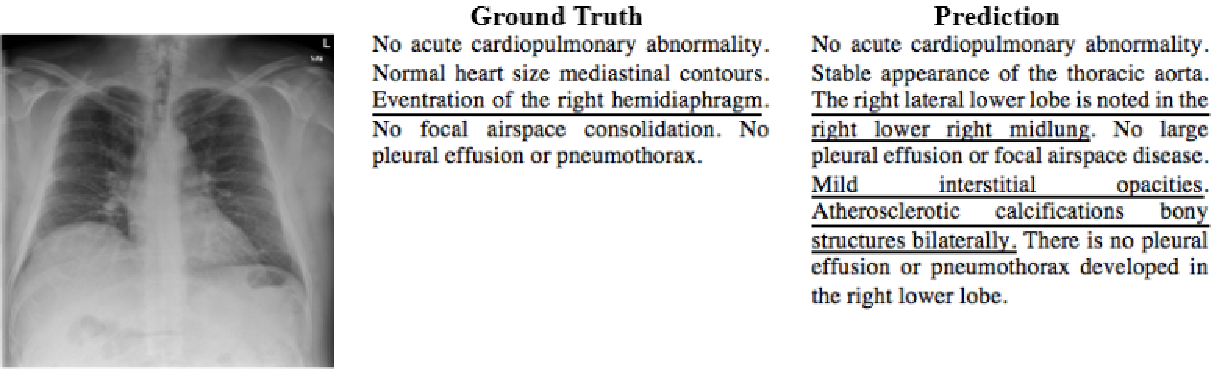
\includegraphics[width=120mm, height=36mm]{../img/ProblemExample}
\caption{Example of an X-ray image along with its ground truth and predicted report. \citet{jing2017automatic}.}
\label{fig01:ProblemExample}
\end{figure}

\section{Methods of generation}
\label{sec:methodsOfGeneration}
In the first part of the analysis, we will present posssible approaches for image caption generation. Inasmuch as almost all solutions for image captioning based on neural networks are using an encoder-decoder architecture as their core with further minor or major adjustments, we will discuss just this architecture. Encoder serves for the purposes of extracting visual features from the input images into intermediate vector representations for the decoder. The decoder is subsequently fed with these visual feature vectors and decodes them token by token into the natural language text.\\

Moreover, over the past years the encoder-decoder architecute has been enhanced using the attention mechanism. The problem of encoder-decoder architecture without any other mechanism is that all the information about the image have to be encoded globally inside a single vector. However, not all the information about the image is relevant for the caption generation. For this reason, the attention mechanism was introduced. Instead of a single vector, the set of feature vectors representing the spatial information of the input image is used. This allows us to dynamically focus only on specific areas during the generation. The overall nature of the mechanism is derived from the way our brains concentrace on the images.\\

Attention mechanism for image captioning was first introduced in the \citet{xu2015show} work using the Bahdanau attention proposed in \citet{bahdanau2014neural}. After extractions of visual feature vectors $h_j$ from image, we want to assign a weight $\alpha_{ij}$ to each of these vectors indicating the relevance of the image position $j$ when generating output at position $i$. This results in the context vector $c_i$, a dynamic weigthed combination of $h_j$ features, that is presented as another input to the decoder. All attention calculations are defined as follows:
\begin{equation}\label{eq01:AttContext}
	c_i = \sum_{j=1}^{t} \alpha_{ij} h_j
\end{equation}

\begin{equation}\label{eq01:AttWeights}
	\alpha_{ij} = \frac{\exp(e_{ij})}{\sum_{k=1}^{t} \exp(e_{ik})}
\end{equation}

\begin{equation}\label{eq01:AttFeedForwardNetwork}
	e_{ij} = a(s_{i-1}, h_j)
\end{equation}

where $s_{i-1}$ is a previous hidden state and $a(s_{i-1}, h_j)$ is an attention model.

\subsection{Encoder}
Encoder is responsible for extracting high-level visual features of the input image into one or more visual feature vectors. Moreover, the encoder can include also additional parts for other independent purposes, e.g. detection of objects in the image and their classification, which may be further passed to the decoder as a separate or an extra input. We will describe some of the most used neural network architectures utilized as an encoder.

\subsubsection{Convolutional neural networks}
Convolutional neural networks (CNN)\citep{o2015introduction} are the most leveraged type of neural networks for the purposes of image analysis. They apply 2D convolution filters for all positions in the image with the shared weights allowing to detect similar patterns independently on the position. Each layer of filters will downsize the dimensions of the previous layer and increases the number of filters. By gradually applying filters, the network is learning more complex patterns.\\

Instead of training convolutional neural networks from scratch, already pretrained CNN models are often used and possiblly further fine-tuned to a specific area. These models have been trained on a vast amount of data thanks to which they learned to recognize relevant features in the lower layers applicable to any kind of images. In contrast, training from scratch is costly and takes a much longer time. Among the used pre-trained CNN model architectures are for example ResNet\citep{he2016deep}, VGGnet\citep{simonyan2014very}, DenseNet\citep{huang2017densely} or EfficientNet\citep{tan2019efficientnet}.

\subsubsection{Transformers}
\label{sec:transformersEncoder}
With the work of \citet{vaswani2017attention}, a new neural network archtecture called tranformers was introduced. The transformers use multi-head self-attention mechanism to compute the relations between the elements in the sequences. Although the transformers were originally designated for NLP tasks, they can be also utilized for other domains like images due to their robustness. Vision transformers (ViT), presented in \citet{dosovitskiy2020image}, is an adaptation of transformers encoder for image classification without any CNNs. The core of the encoder is identical to the one in the original transformer. Nevertheless, the input image is represented as a sequence of patches for which their embeddings are computed together with the positional encodings as the input, as we can see in the Figure \hyperref[fig02:ViT]{1.2}.

\begin{figure}[h]\centering
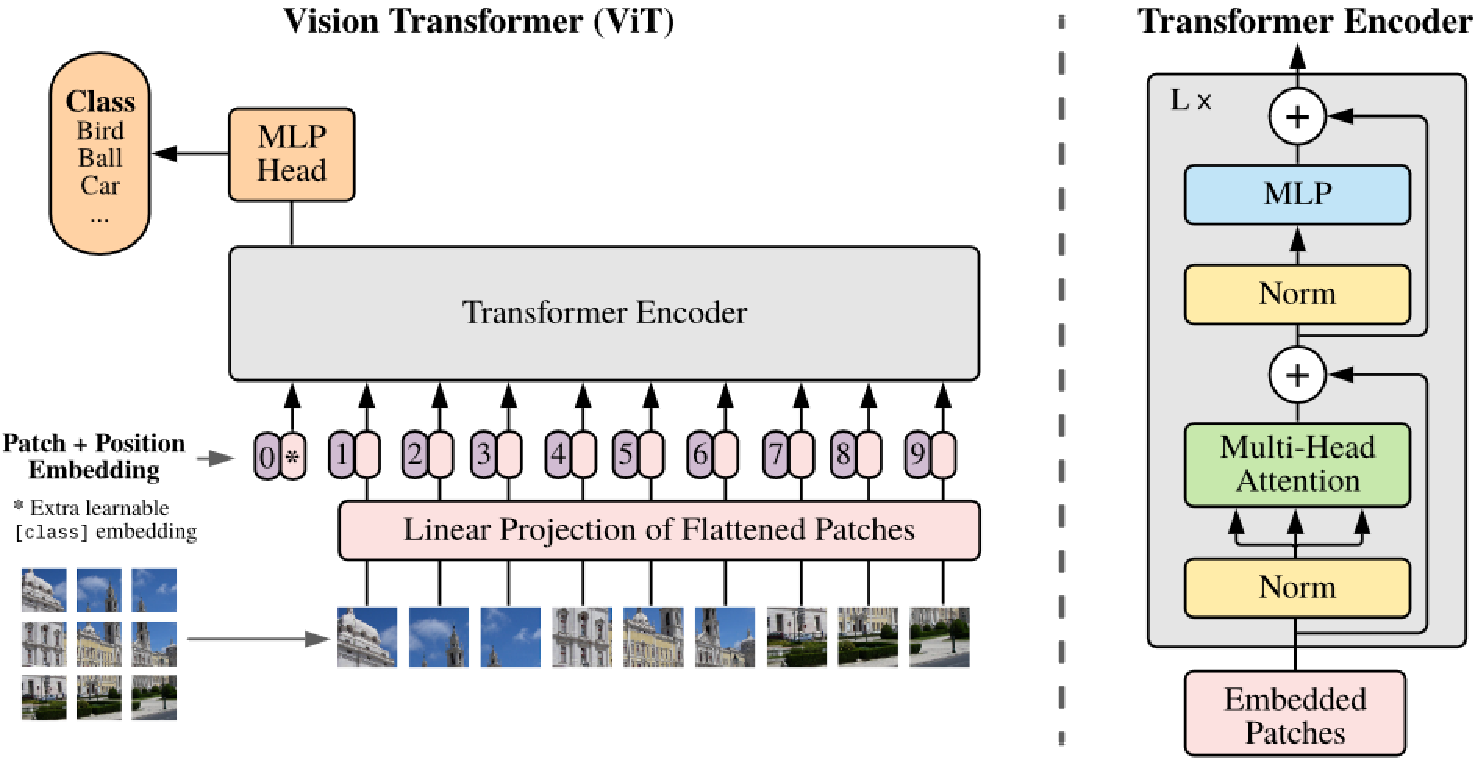
\includegraphics[width=145mm, height=76mm]{../img/VisualTransformerArchitecture}
\caption{Visual Transformer architecture from \citet{dosovitskiy2020image}.}
\label{fig02:ViT}
\end{figure}

\subsection{Decoder}
The second main part of the network is the decoder which serves as a language model for generating corresponding captions to input images. During the generation process the visual features of the image from the encoder and the already generated text are taken into account for the predtiction of the next token or word. In the process of generation, the attention mechanism (described above in the Chapter \ref{sec:methodsOfGeneration}) is almost always incorporated in order to focus only on the substantial particular areas. The following subsections present common approaches used as the backbones for the decoder part of the network.
\subsubsection{Recurrent neural networks}
Recurrent neural networks (RNN)\citep{rumelhart1985learning} are a category of neural networks designated for sequence data processing. Context of the previous part of the sequence can influnence the subsequent elements due to the RNN cell's internal memory (hidden state). Each time step RNN cell computes its activation function from current input and hidden state producing updated hidden state as output. For language modeling tasks, the last generated token or word is given to the RNN as the next input until the entire text is produced. The autoregressiveness of the RNNs is the reason why they are ideal for use as a language model. The two most used types of RNN cells are LSTM\citep{hochreiter1997long} and GRU\citep{cho2014learning}, however the LSTM cells are more utilized as the decoder because they can remember longer sequences. Moreover, we can combine them in a hierarchical manner to capture more complex structures in the generated text. Neverthless, the downside of the RNNs is the training time due to their sequential nature. The whole sentence must pass through RNN token by token and cannot be parallelized. In addition, due to the sequential pass of the input, there is also another serious problem - the RNN may forget the information about earlier  elements on long sequences because of the vanishing gradient.

\subsubsection{GPT-2}
Just as in the case of encoder, with the advent of transformers presented in the \citet{vaswani2017attention} paper, the decoder part of transformers started to be used as the language model for image captioning task for their great results in the natural language processing (NLP) tasks. One of the advantages of the transformers against the previously used recurrent neural networks is the loss of the need for sequential processing during the training. Due to the fact that the processing of the whole caption can be done in parallel, the entire training process is significatnly accelerated. Moreover, the transformers can capture longer ranges dependencies in the text, as they process the sentence as a whole instead of sequentially by words.\\

One of the state-of-the-art autoregressive language models using transformers as their backbone is OpenAI GPT-2 model from the \citet{radford2019language} paper, which outperforms other language models on many NLP tasks. It was trained on a massive English dataset called WebText (introduced in the same article) containing a total of 40 GB of raw text. The resuling model is able to generate large coherent texts. Furthermore, it can be fine-tuned to a different domain or to a completely different language.

\section{Data}
In the previous part, we talked about possible methods of generation. Another crucial aspect we need to discuss are data, which are a basic building block of our thesis. This part focuses on the analysis of the data we used in our thesis, but also on their alternatives. \\

In order to solve our task and train neural network, we need to get dataset containing the X-rays images along with their textual descriptions and optionally some other attributes of the examined X-rays. Moreover, the fundamental feature we need is that the data must be in the Czech language.

\subsection{Existing datasets}
\label{sec:datasets}
Medical environment provides a plenty of diverse potential problems, which can be researched. As already mentioned, in this thesis we focus specifically on the X-ray images. Because it is not so hard to detect fractures on the limbs, this area is not as interesting as others. One area that is rich in its diversity is the chest. As a result, this area is explored the most and therefore there exist multiple datasets with full textual medical reports. In the following section we describe some of them.\\

\subsubsection{Indiana University chest X-ray}
\label{sec:IUDataset}
Indiana University chest X-ray dataset has become a standard in the field of medical report generation. It was presented in the \citet{10.1093/jamia/ocv080} paper. This dataset is an open source collection of pairs of chest X-rays and their corresponding semi-stuctured textual radiology reports, which is freely available on the web\footnote[1]{\url{https://openi.nlm.nih.gov/faq\#collection}} without any additional requirements. We have a choice if we want to download just reports or images and in either PNG or DICOM\footnote[2]{\url{https://www.dicomstandard.org/}} format. The entire dataset consists of 7470 chest X-ray images that cover not only the frontal (PA\footnote[3]{Posterior-Anterior}) view, but also the lateral (side) one. These images corresponds to a total of 3995 patients' medical text reports.\\

Figure \hyperref[fig03:IUChestXRaySample]{1.3} shows an example from the Indiana University chest X-ray dataset. Each dataset pair is carefully de-identified in order to remove any personal information. The text of the report is semi-structured in up to 5 sections. The most important sections are \textit{impression}, where the overall diagnosis is stated, \textit{findings} section describing the details of examination and \textit{tags} which are of two types - manual and automatic. Manual tags were annotated manually using MeSH\footnote[4]{\url{https://www.nlm.nih.gov/mesh/meshhome.html}} and RadLex\footnote[5]{\url{http://radlex.org/}} codes, automatic were encoded from the reports using the MTI~indexer.\footnote[6]{\url{https://lhncbc.nlm.nih.gov/ii/tools/MTI.html}} The rest of the sections are \textit{indication} and \textit{comparison}.\\

The disadvantage of this dataset is that it is relatively small. On the other hand, it is a quite clean and manually checked dataset containing also additional information about images in a form of tags described above.

\begin{figure}[h]\centering
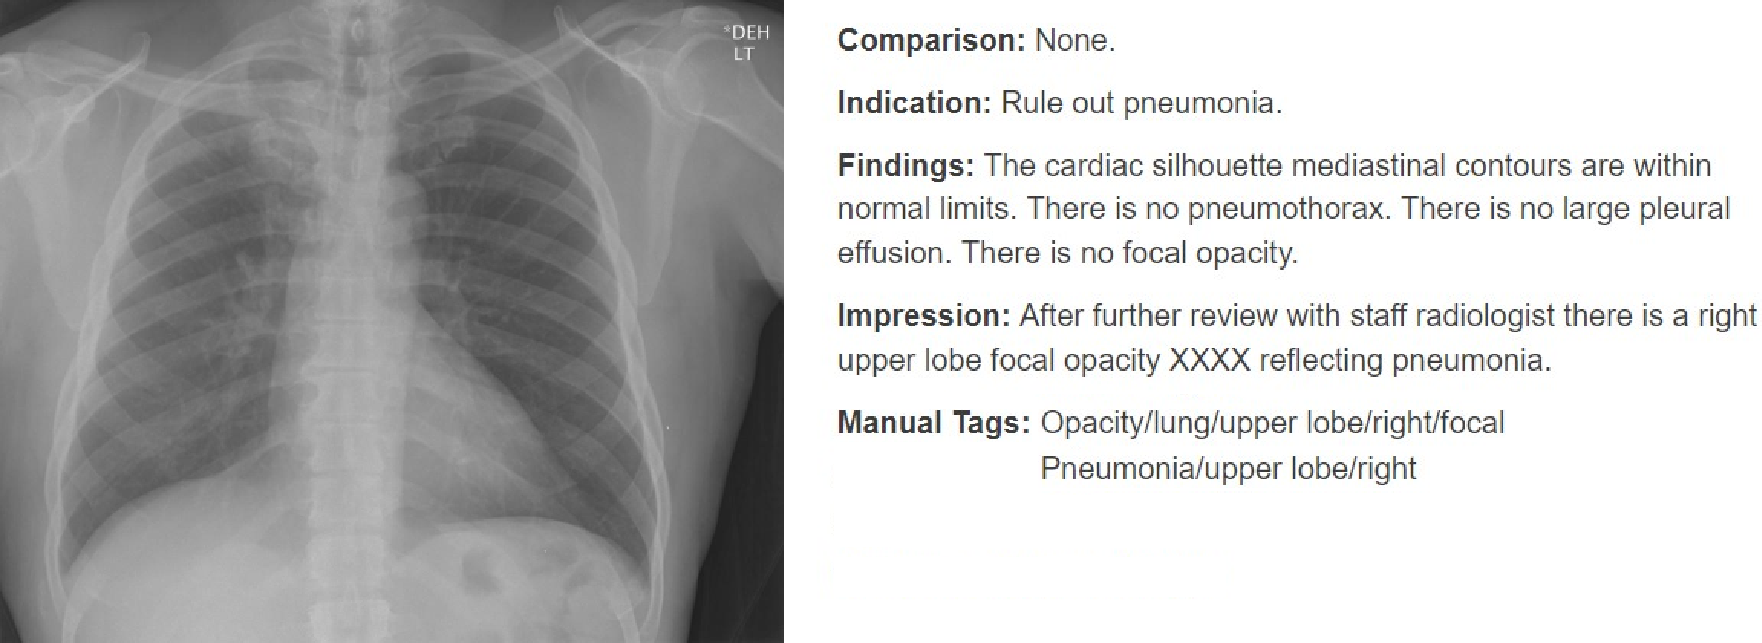
\includegraphics[width=145mm, height=53mm]{../img/IUChestXRaySample_CXR1728_IM-0479-1001}
\caption{Sample from the Indiana University Chest X-ray dataset.}
\label{fig03:IUChestXRaySample}
\end{figure}

\subsubsection{MIMIC-CXR v2.0.0}
MIMIC-CXR v2.0.0 is another dataset consisting of full semi-structured medical textual reports against corresponding chest X-rays that was presented in the \citet{cxr:johnson2019mimic} paper. As the previous dataset, it is openly available on the web\footnote[7]{\url{https://physionet.org/content/mimic-cxr/2.0.0/}}. In order to get access to the dataset, we have to go through registration and verification steps. The verification phase includes completion of CITI\footnote[8]{\url{https://about.citiprogram.org/series/human-subjects-research-hsr/}} \textit{Data or Specimens Only Research} course for \textit{Human Subject Research}. Moreover we need somebody trustworthy as a reference to confirm the authenticity of our identity. After the verification we get access to all datasets in the same repository.\\

The dataset consists of 377,110 X-ray images in the DICOM format connected to a total of 227,835 radiology reports for 65,379 patients. Each report is structured into multiple different sections as we can see in the Figure \hyperref[fig04:MimicCXRSample]{1.4}. In order to satisfy legal requirements, entire dataset is automatically de-identified to remove any protected~health~information.\footnote[9]{\url{https://en.wikipedia.org/wiki/Protected\_health\_information}} Similarly to the previous dataset, the essential two sections of each report are \textit{impression} and \textit{findings}. There also exists older MIMIC-CXR-JPG\footnote[10]{\url{https://physionet.org/content/mimic-cxr-jpg/2.0.0/}} dataset, presented in the \citet{cxr-jpg:johnson2019mimic} paper. This is an older version of MIMIC-CXR v2.0.0 dataset consisting of the exactly same images, only in JPG format, but each image is assigned 14 labels indicating the presence of the category in the report instead of its textual form. Each category has assigned either a \textit{1}, \textit{0} or \textit{-1} label with the meaning \textit{positively mentioned}, \textit{negatively mentioned} or \textit{uncertain}. The labels were determined from the reports utilizing the CheXpert\citep{irvin2019chexpert} and the NegBio\citep{peng2018negbio} open-source labelers.\\

The advantage of this dataset is its vast number of samples. Moreover, as described above, we can get additional information in a form of categories to every image. Nevertherless, the textual reports carry some noise in them in the form of grammatical mistakes and incorrect formatting. We face these issues in the Chapter \ref{sec:DataPreprocessing}. 

\begin{figure}[h]\centering
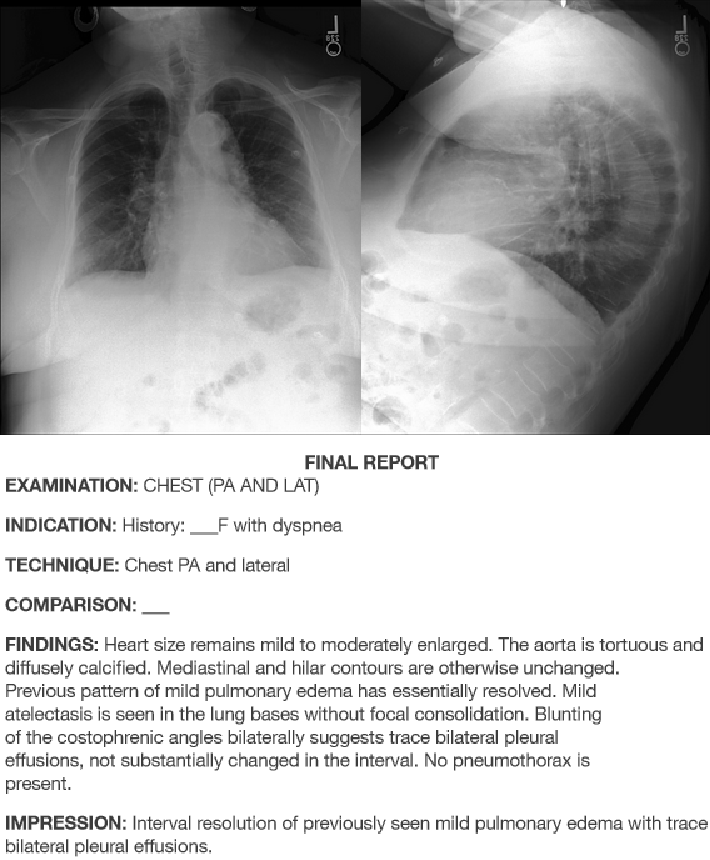
\includegraphics[width=135mm, height=163mm]{../img/mimic_s57861150}
\caption{Sample from the MIMIC-CXR dataset.}
\label{fig04:MimicCXRSample}
\end{figure}

\subsubsection{Other datasets}
Apart from the datasets described above, other datasets with similar type are being used with the aim of solving our task. Amongst them belong datasets such as ImageCLEFmed~Caption\citep{ImageCLEFmedicalCaptionOverview2022}, PadChest\citep{bustos2020padchest}, BCIDR\citep{zhang2017mdnet} and PEIR~Gross\citep{jing2017automatic}. Moreover, except for datasets containing textual reports there exist a lot of other datasets worth mentioning containing different kind of information for each X-ray. These include, for example, CheXpert\citep{irvin2019chexpert}, VinDr-CXR\citep{nguyen2020vindr}, ChestX-ray8\citep{wang2017chestx} and its expanded version ChestX-ray14.

\subsection{Czech data}
\label{sec:CzechData}
All freely available datasets presented in the previous part have one common downside, namely they are not in the Czech language. As a part of elaboration of this thesis, an intesive communication with real Czech hospitals and other possible sources of real data took place. The goal of this communication was to create the very first open Czech dataset of this kind. Processing of this kind of data would mean not only preparing the data into suitable format but also it would include proper anonymization of any personal information about the patients within the data. \\

However, inasmuch as the authentic patients data from hospitals are subject to strict privacy rules and we are not employees of any hospital, the institutions decided that they cannot provide the data in any way without the concious permission of patients given before the examination. With this result, we need to find a different way how to obtain this much needed Czech data.

\subsection{Translators}
\label{sec:Translators}
In the previous sections, we discovered that there is no dataset in the Czech language for our problem and there is no easy way how to get acces to the real data in order to build one. The only thing left is to create a new artificial dataset using an automatic or manual translation. Manual translation would be expensive, time consuming and would require proper domain knowledge. Therefore, we will compare different freely accessible translators and choose the right one for our needs.

\subsubsection{DeepL}
At the moment, DeepL\footnote[11]{\url{https://www.deepl.com/translator}} translator provides the finest available translations beating even the ones from Google Translate. Moreover, it has freely usable web application and REST API. However, the main drawback of the DeepL translator is that its REST API is highly limited - only 500 000 characters per month can be translated for free. Furthermore, any translation above this limit is costly and thus this path is not appropriate for translating large textual datasets.

\subsubsection{Google Translate}
Google~Translate\footnote[12]{\url{https://translate.google.com/}} has become already de facto standard in the world of machine translation and it is the most used freely accessible language translation service in the world. In terms of quality, the translations are still great although little bit worse than those from DeepL. The web application is free of any charge and anybody can use it as much as he needs. Nevertheless, just as in the case of DeepL, their REST API services are limited and translation of anything above that limit is expensively charged. For these reasons, as in the previous case, we must find another way.

\subsubsection{CUBBITT}
\label{sec:Cubbitt}
Machine~Translation\citep{akhbardeh2021findings} is an extensive area of research, as a result of which there exist many other projects and academic papers nowadays. One of them is CUBBITT\footnote[13]{\url{https://lindat.mff.cuni.cz/services/translation/}} translator, which was developed at our faculty. The whole system is presented and described in detail in the \citet{biblio:PoToTransformingmachine2020} paper. \\

CUBBITT translator provides translations which are comparable to the ones from DeepL and Google Translate services. As other mentioned translators it provides an openly available web application for machine translation. Moreover and most importantly it provides REST API that is practically unlimited in text volume and free to use without any additional charges. These are the reasons why we will utilize CUBBITT in our thesis as a translator to create our artificial dataset.\\

On the other hand, CUBBITT has no support for auto-correcting input text compared to above mentioned services. Moreover, there are some patterns in the text which CUBBITT cannot translate at all or translates them incorrectly. These problems complicates our situation as the data from hospitals carry some natural noise in them. We face these complications in Chapter \ref{sec:DataPreprocessing}.

\section{Related work}
\label{sec:RelatedWork}
The last section of this chapter is dedicated to the description and comparison to some of the related works that solve identical or similar problem as we do.\\

The most significant related work is \citet{alfarghaly2021automated} inasmuch as we base our thesis on it. This paper focuses on the identical problem as we do, only in the English language. The proposed solution uses a pre-trained and further fine-tuned Chexnet model, presented in \citet{rajpurkar2017chexnet}, as a visual features encoder and distilGPT2\footnote[14]{\url{https://huggingface.co/distilgpt2}} language model\citep{sanh2019distilbert} as a decoder which is additionally conditioned on the visual features and predicted tag's word2vec\citep{mikolov2013distributed} embeddings. For training the neural network the Indiana University chest X-ray dataset, described in more detail in Chapter \ref{sec:IUDataset}, is used. Figure \hyperref[fig05:OmarExample]{1.5} shows examples of the model outputs.\\

\begin{figure}[h]\centering
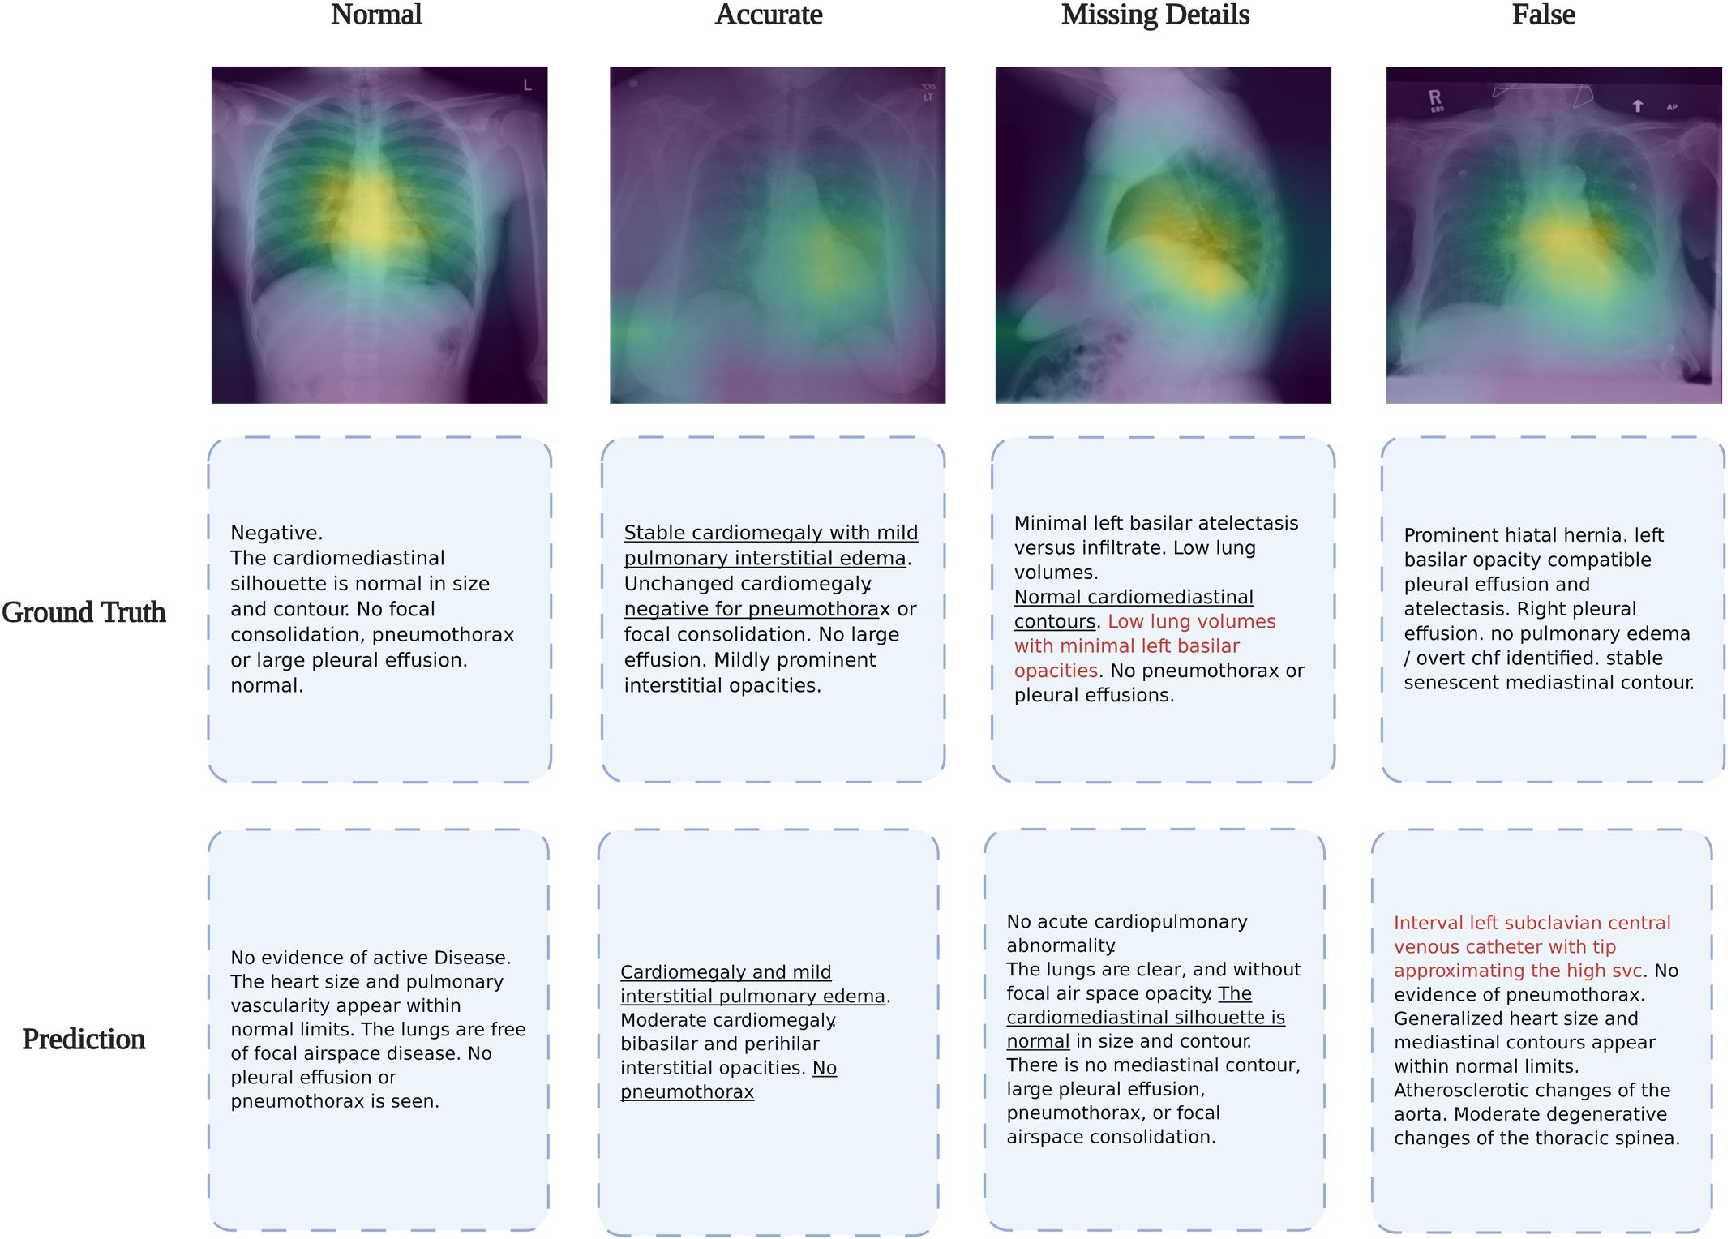
\includegraphics[width=145mm, height=104mm]{../img/OmarExample}
\caption{Examples of generated medical reports from \citet{alfarghaly2021automated}.}
\label{fig05:OmarExample}
\end{figure}

Another paper making use of transformers is \citet{chen2020generating}. The visual features of images are extracted using pre-trained convolutional neural network and they are further passed to the transformer encoder outputting hidden states, that are further presented to the transformer decoder for the report generation. However, the decoder architecture contains special memory module and also enhances the layer normalization. The memory module serves for memorization of text patterns which occur in the similar images inasmuch as they can further help for generating the report. We can see its effect in the Figure \hyperref[fig06:ZhihongExample]{1.6}. Indiana University chest X-ray and MIMIC-CXR v2.0.0 datasets (see Chapter \ref{sec:datasets} for more details) were used as training data.\\

\begin{figure}[h]\centering
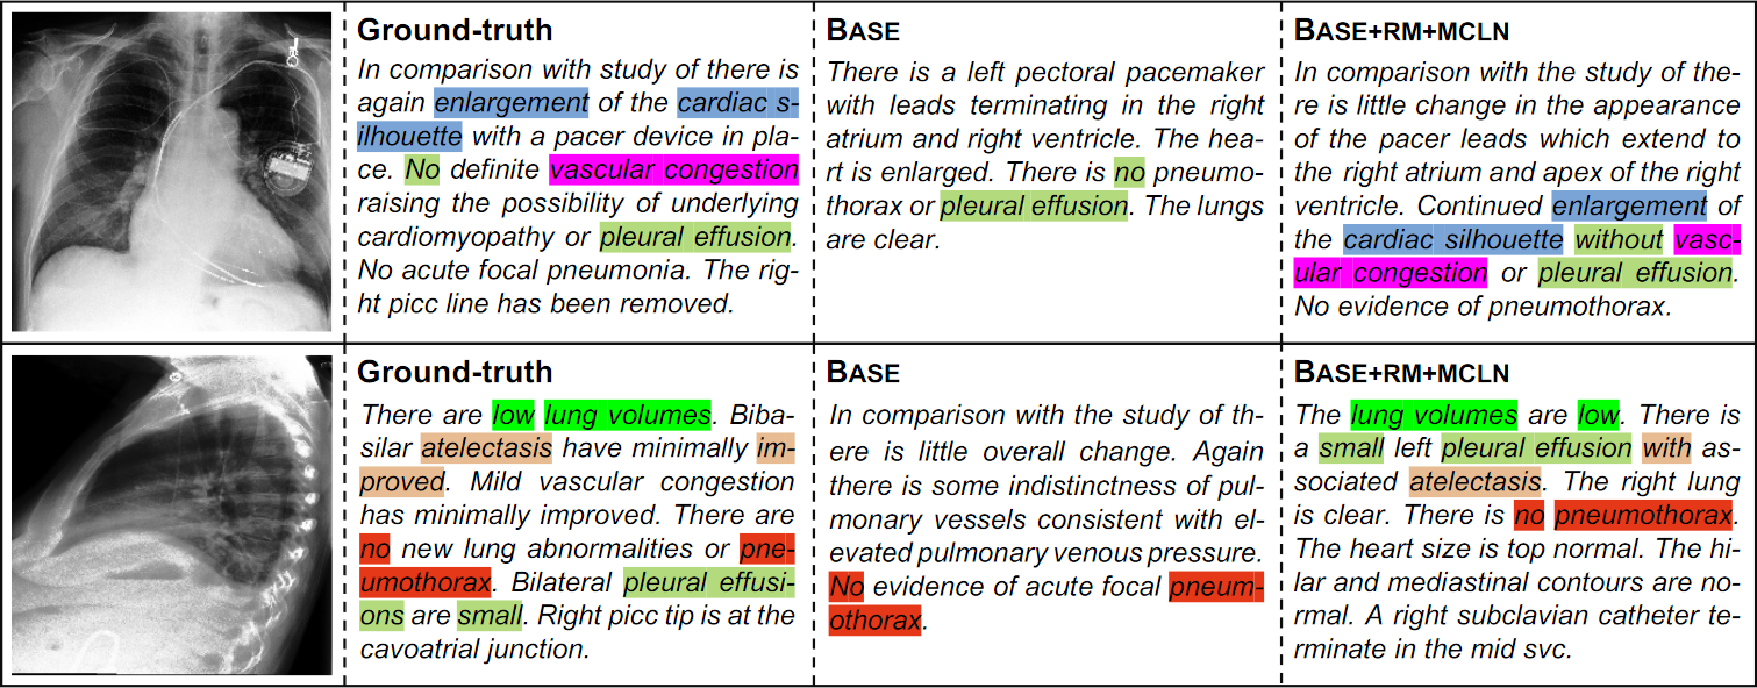
\includegraphics[width=145mm, height=57mm]{../img/ZhihongExample}
\caption{Examples of generated medical reports from \citet{chen2020generating}.}
\label{fig06:ZhihongExample}
\end{figure}

\citet{yuan2019automatic} paper proposes a hiearchical encoder-decoder architecture as we can see in the Figure \hyperref[fig07:YuanExample]{1.7} for the purpose of generating textual reports. Pairs of frontal and lateral X-ray images are used as an input to the network instead of single images, as the authors claim that the images should be complementary to each other instead of being processed independently. The RestNet-152 model pre-trained on the CheXpert\citep{irvin2019chexpert} dataset is utilized as the encoder with three outputs used later - the global and local features of the images, predicted observations and medical concepts. The decoder is hierarchical LSTM decoder comprising of the two parts: \textit{sentence decoder} and \textit{word decoder}. The sentence decoder takes visual features and generates hidden state for each sentence, which are along with the predicted medical concepts presented to the word decoder in order to generate the report. There are many other papers using a hierarchical architecture, e.g. \citet{huang2019multi}. \\

\begin{figure}[h]\centering
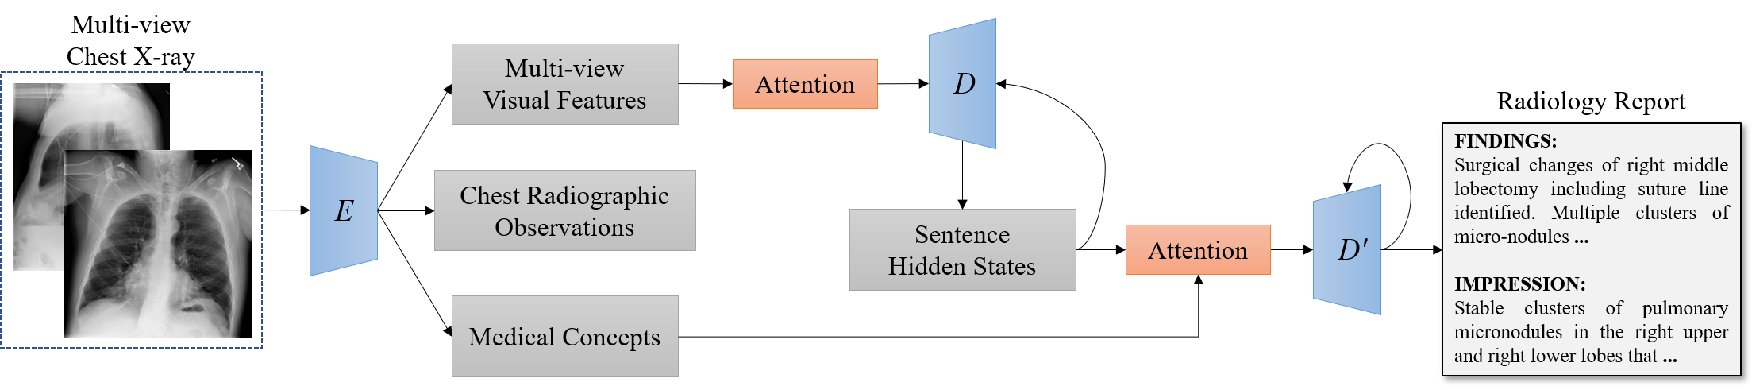
\includegraphics[width=145mm, height=32mm]{../img/YuanExample}
\caption{Hierarchical architecture from \citet{yuan2019automatic}.}
\label{fig07:YuanExample}

\textit{E} is encoder, \textit{D} is sentence decoder and \textit{D\textquotesingle} is word decoder.
\end{figure}

The last related project we mention in this work is CareBot,\footnote[15]{\url{https://www.carebot.com/}} which is being developed concurrently with our thesis. CareBot is a Czech startup founded in 2021 as a reaction to the then ongoing Covid-19 pandemic. As in our work, CareBot focuses its attention mainly on the processing of chest X-rays using neural networks. However, unlike us, it does not generate the textual reports for the doctors. Instead of textual reports, it focuses on finding and classifying a total of 15 different types of individual diseases on X-ray images and their subsequent spatial localization. Moreover, they already have a support from the medical environment. In their related papers \citep{kvak2022towards} and \citep{kvak2021carebot} they as Resnet50V2 and DenseNet121 as the backbone atchitectures. However, their final architecture and methodolgy have not been publushed anywhere yet.











